\documentclass[11pt,a4paper]{article}
\usepackage[utf8]{inputenc}
\usepackage[spanish,es-tabla]{babel}
\usepackage{geometry}
\geometry{margin=2.5cm}
\usepackage{amsmath}
\usepackage{amsfonts}
\usepackage{amssymb}
\usepackage{graphicx}
\usepackage{hyperref}
\usepackage{titlesec}
\usepackage{enumitem}
\usepackage{booktabs}
\usepackage{listings}
\usepackage{xcolor}
\usepackage{float}

\definecolor{codegreen}{rgb}{0,0.6,0}
\definecolor{codegray}{rgb}{0.5,0.5,0.5}
\definecolor{codepurple}{rgb}{0.58,0,0.82}
\definecolor{backcolor}{rgb}{0.96,0.96,0.94}

\lstset{
    backgroundcolor=\color{backcolor},   
    commentstyle=\color{codegreen},
    keywordstyle=\color{blue},
    numberstyle=\tiny\color{codegray},
    stringstyle=\color{codepurple},
    basicstyle=\ttfamily\footnotesize,
    breakatwhitespace=false,         
    breaklines=true,
    captionpos=b,                    
    keepspaces=true,                 
    numbers=left,                    
    numbersep=5pt,                  
    showspaces=false,                
    showstringspaces=false,
    showtabs=false,                  
    tabsize=2,
    literate={á}{{\'a}}1 {é}{{\'e}}1 {í}{{\'i}}1 {ó}{{\'o}}1 {ú}{{\'u}}1
             {Á}{{\'A}}1 {É}{{\'E}}1 {Í}{{\'I}}1 {Ó}{{\'O}}1 {Ú}{{\'U}}1
             {ñ}{{\~n}}1 {Ñ}{{\~N}}1 {ü}{{\"u}}1 {Ü}{{\"U}}1
}

\title{\textbf{Proyecto Final: Sistema de Gestión de Tienda Online}}
\author{\textbf{Joanthan Jesús Flores Reyes} \\ Universidad Autónoma Metropolitana, Unidad Cuajimalpa}
\date{\today}

\begin{document}

\maketitle
\tableofcontents
\newpage

\section{Introducción al Problema y Objetivos}
En este proyecto se aborda el diseño y la implementación de una base de datos relacional orientada a una tienda en línea especializada en la venta de productos electrónicos. El propósito principal es desarrollar un sistema estable, consistente y bien estructurado que permita gestionar de manera eficiente toda la operación diaria del negocio, abarcando desde el control estricto de inventarios hasta el seguimiento detallado de clientes, pedidos y opiniones de los compradores.

\subsection{Objetivos del Proyecto}
\begin{itemize}[label=$\bullet$]
    \item \textbf{Diseño Estructurado:} Modelar un esquema relacional sólido que interconecte de forma óptima las entidades esenciales del sistema: Clientes, Productos, Categorías, Pedidos, Detalles de Pedido y Reseñas.
    \item \textbf{Implementación de Reglas de Negocio:} Restringir el comportamiento de los datos mediante reglas operativas directo en el SGBD (MySQL). Esto incluye asegurar que el stock nunca sea negativo, limitar a los clientes a un máximo de 5 pedidos pendientes y validar que solo los compradores reales puedan dejar reseñas sobre un producto.
    \item \textbf{Automatización y Optimización:} Crear consultas avanzadas y un conjunto de 8 procedimientos almacenados para automatizar los procesos clave, optimizando el rendimiento general mediante índices estratégicos y validando la integridad del sistema con un lote completo de datos de prueba.
\end{itemize}

\section{Análisis y Diseño del Modelo}

\subsection{Diagrama Entidad-Relación (ER)}
Para dar solución a los requerimientos de la tienda, estructuramos el modelo mediante un esquema de 6 tablas interconectadas. Esto garantiza una separación clara de responsabilidades y facilita el mantenimiento y escalabilidad a largo plazo.

\begin{figure}[H]
    \centering
    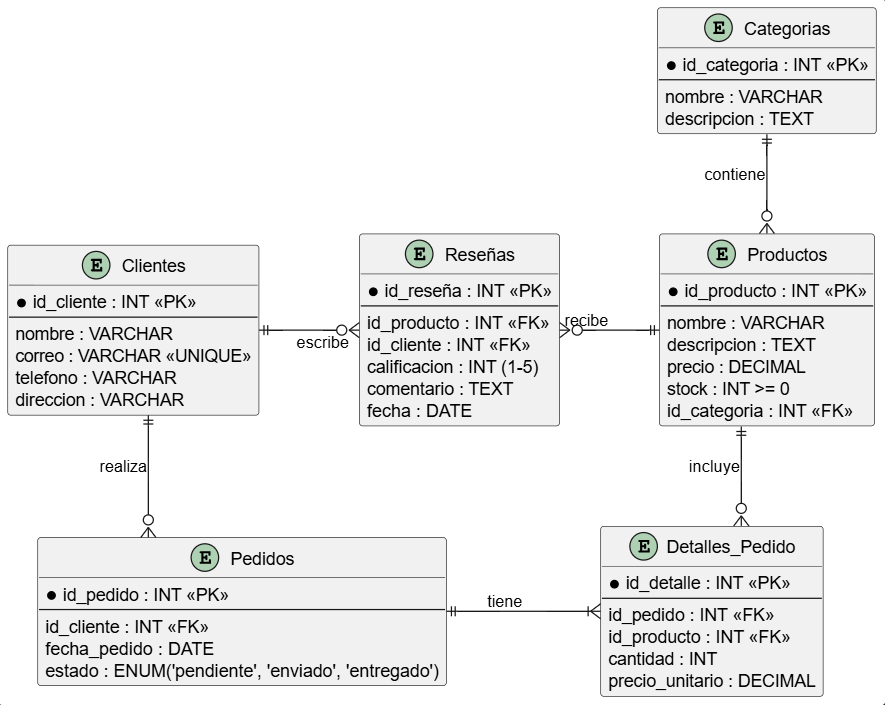
\includegraphics[width=0.8\textwidth]{DER.png}
    \caption{Esquema conceptual del modelo Entidad-Relación de la tienda electrónica.}
    \label{fig:diagrama_er}
\end{figure}

\subsection{Definición de Claves y Relaciones}
Para asegurar la consistencia y la integridad referencial de la información, se definieron con precisión las llaves dentro de nuestro modelo:
\begin{itemize}
    \item \textbf{Claves Primarias (PK):} Cada entidad cuenta con un identificador único auto-incremental para indexar los registros de forma eficiente: \texttt{id\_cliente}, \texttt{id\_producto}, \texttt{id\_categoria}, \texttt{id\_pedido}, \texttt{id\_detalle} e \texttt{id\_reseña}.
    \item \textbf{Claves Foráneas (FK):} Establecen los vínculos relacionales y las restricciones de integridad entre las tablas:
    \begin{itemize}
        \item \texttt{id\_categoria} en Productos (relaciona cada artículo con su respectiva familia o categoría).
        \item \texttt{id\_cliente} en Pedidos y Reseñas (asocia las compras y los comentarios con el usuario correspondiente).
        \item \texttt{id\_pedido} e \texttt{id\_producto} en Detalles\_Pedido (desglosa cada uno de los artículos que componen una orden).
        \item \texttt{id\_producto} en Reseñas (vincula la calificación y comentario directamente con el artículo adquirido).
    \end{itemize}
    \item \textbf{Claves Candidatas:} El atributo correo en la tabla Clientes se define con una restricción de unicidad (UNIQUE), funcionando como una clave alternativa ideal para identificar a cada usuario de forma única en el sistema.
\end{itemize}

\subsection{Justificación de la Normalización (3NF)}
El diseño de la base de datos se estructuró siguiendo los principios de la Tercera Forma Normal (3NF) para garantizar la integridad de los datos, evitar la redundancia masiva y prevenir anomalías al actualizar o borrar información. A continuación se detalla cómo el modelo cumple con cada regla:
\begin{enumerate}
    \item \textbf{Primera Forma Normal (1NF) - Atributos atómicos:} 
    Esta regla dicta que cada celda de una tabla debe contener un único valor indivisible. En el contexto de la tienda, un cliente puede comprar varios artículos en una sola orden. En lugar de almacenar una lista separada por comas (por ejemplo: "Monitor, Teclado, Ratón") en una sola celda dentro de la tabla \textit{Pedidos}, se estructuró la tabla independiente \textit{Detalles\_Pedido}. De esta manera, cada artículo comprado se registra en su propia fila de forma atómica y limpia.
    \item \textbf{Segunda Forma Normal (2NF) - Dependencia funcional completa:} 
    Además de cumplir con la 1NF, todos los atributos que no son clave deben depender por completo de la clave primaria. Por ejemplo, en la tabla \textit{Detalles\_Pedido}, si incluyéramos el nombre del producto, ese nombre dependería únicamente del \texttt{id\_producto} y no del pedido en sí. Para evitar esta dependencia parcial, toda la información descriptiva del artículo se mantiene exclusivamente en la tabla \textit{Productos}.
    \item \textbf{Tercera Forma Normal (3NF) - Sin dependencias transitivas:} 
    Estando en 2NF, ningún atributo no clave debe depender de otro atributo no clave. El mejor ejemplo en nuestro esquema es la separación entre \textit{Productos} y \textit{Categorías}. Si almacenáramos el nombre y la descripción de la categoría directamente en la tabla \textit{Productos}, estos datos dependerían de la categoría y no del producto directamente. Al aislar esta información en la tabla \textit{Categorías}, evitamos repetir el mismo texto descriptivo cientos de veces en el catálogo. De este modo, si la tienda decide modificar el nombre de una categoría, la actualización se realiza en un solo registro y se propaga de forma automática a todos los productos relacionados.
\end{enumerate}

\section{Implementación de la Base de Datos}
La base de datos fue construida en el SGBD MySQL. Todo el proceso fue dividido en scripts secuenciales que garantizan la correcta creación de la estructura, la inserción de datos de prueba (30 productos, 15 clientes, 20 pedidos y 10 reseñas) y la programación de la lógica de negocio a través de procedimientos almacenados.

Los scripts desarrollados se encuentran alojados en el repositorio del proyecto e incluyen la creación de las tablas con sus respectivas restricciones (\texttt{CHECK} y \texttt{UNIQUE}), así como los índices estratégicos para acelerar el procesamiento de datos.

\section{Validación y Optimización}

\subsection{Resultados de las Consultas Analíticas}
Al ejecutar las vistas analíticas sobre el lote de datos de prueba, el sistema generó los siguientes reportes:

\textbf{Consulta 1: Productos disponibles por categoría (Muestra parcial)} \\
La consulta agrupó y ordenó correctamente el catálogo de menor a mayor precio dentro de cada categoría.
\begin{table}[H]
    \centering
    \footnotesize
    \begin{tabular}{@{}llrr@{}}
        \toprule
        \textbf{Categoría} & \textbf{Producto} & \textbf{Precio (\$)} & \textbf{Stock} \\
        \midrule
        Almacenamiento & Gabinete Externo Orico para SSD & 450.00 & 35 \\
        Audio & Audífonos Inalámbricos Xiaomi & 850.00 & 50 \\
        Componentes PC & Pasta Térmica de Alto Rendimiento & 200.00 & 100 \\
        Monitores & Monitor de Oficina 24" FHD & 2200.00 & 15 \\
        Periféricos & Mouse Pad RGB Extendido & 350.00 & 100 \\
        \bottomrule
    \end{tabular}
\end{table}

\textbf{Consulta 2: Clientes con pedidos pendientes y total histórico} \\
El reporte filtró exitosamente a los usuarios que tienen órdenes en estado "pendiente" y calculó su gasto total de compras.
\begin{table}[H]
    \centering
    \footnotesize
    \begin{tabular}{@{}llrr@{}}
        \toprule
        \textbf{Nombre} & \textbf{Correo} & \textbf{Pedidos Pendientes} & \textbf{Total Gastado (\$)} \\
        \midrule
        Jorge Salinas & jorge.s@email.com & 2 & 9300.00 \\
        Daniela Torres & dany.t@email.com & 1 & 900.00 \\
        Fernando Silva & fer.silva@email.com & 1 & 8900.00 \\
        Hugo Morales & hugo.m@email.com & 1 & 3100.00 \\
        \bottomrule
    \end{tabular}
\end{table}

\textbf{Consulta 3: Top 5 productos con mejor calificación} \\
El sistema promedió correctamente las calificaciones dejadas por los usuarios en el catálogo.
\begin{table}[H]
    \centering
    \footnotesize
    \begin{tabular}{@{}lrr@{}}
        \toprule
        \textbf{Producto} & \textbf{Promedio Calificación} & \textbf{Total Reseñas} \\
        \midrule
        Tarjeta Gráfica AMD Radeon RX 7800 XT & 5.00 & 1 \\
        Monitor Gaming 144Hz 27" & 5.00 & 1 \\
        Audífonos de Estudio Cerrados & 5.00 & 1 \\
        Mouse Gaming Logitech G502 & 5.00 & 1 \\
        Micrófono de Condensador USB & 4.00 & 1 \\
        \bottomrule
    \end{tabular}
\end{table}

\subsection{Resultados de Pruebas de Procedimientos Almacenados}
Para garantizar la integridad del sistema, se ejecutaron pruebas funcionales sobre los 8 procedimientos almacenados, forzando errores de lógica de negocio para comprobar los candados de seguridad. A continuación, las salidas obtenidas:

\textbf{1. Prueba de validación de reseñas (\texttt{sp\_registrar\_reseña}):} \\
Al intentar que un cliente reseñara un producto que no ha comprado, la base de datos bloqueó la inserción y arrojó el error:
\begin{lstlisting}[language=SQL, numbers=none]
Error Code: 45000. Error: Solo los clientes que han comprado el producto pueden dejar una reseña.
\end{lstlisting}

\textbf{2. Prueba de límite de pedidos (\texttt{sp\_registrar\_pedido}):} \\
Se simuló la inserción de un sexto pedido pendiente para un mismo cliente. El procedimiento detuvo la acción con la siguiente alerta:
\begin{lstlisting}[language=SQL, numbers=none]
Error Code: 45000. Error: El cliente ya alcanzó el límite de 5 pedidos pendientes.
\end{lstlisting}

\textbf{3. Actualización de inventario (\texttt{sp\_actualizar\_stock}):} \\
Se ejecutó una simulación de compra descontando 5 unidades de un producto. El sistema restó la cantidad correctamente, actualizando el stock general de 15 a 10 unidades de forma inmediata.

\textbf{4. Cambio de estado de pedido (\texttt{sp\_cambiar\_estado\_pedido}):} \\
Se actualizó exitosamente el estado del pedido ID 5, pasando de \textit{'pendiente'} a \textit{'enviado'}.

\textbf{5. Eliminar reseña y recalcular (\texttt{sp\_eliminar\_reseña}):} \\
Al borrar una calificación del sistema, el procedimiento se ejecutó sin errores y devolvió una tabla virtual mostrando el nuevo promedio de calificación del producto afectado.

\textbf{6. Evitar productos duplicados (\texttt{sp\_agregar\_producto}):} \\
Se intentó registrar un artículo con un nombre ya existente dentro de la misma categoría. El sistema protegió el catálogo arrojando:
\begin{lstlisting}[language=SQL, numbers=none]
Error Code: 45000. Error: Ya existe un producto con el mismo nombre en esta categoría.
\end{lstlisting}

\textbf{7. Actualizar información de cliente (\texttt{sp\_actualizar\_cliente}):} \\
Se modificó exitosamente el número de teléfono y la dirección de envío de un cliente, sin afectar su historial de compras ni su identificador único.

\textbf{8. Reporte de stock bajo (\texttt{sp\_reporte\_stock\_bajo}):} \\
El procedimiento escaneó el inventario y devolvió la tabla con los artículos próximos a agotarse (menos de 5 unidades), mostrando en la columna \texttt{estado\_inventario} el aviso automático: \textit{"¡Cuidado: Stock bajo, requiere reabastecimiento!"}.

\subsection{Impacto de los Índices (Análisis con EXPLAIN)}
El rendimiento de las consultas críticas fue evaluado utilizando el comando \texttt{EXPLAIN} del motor MySQL para medir el impacto directo de los índices implementados:
\begin{itemize}
    \item \textbf{Escenario sin índices (Full Table Scan):} Inicialmente, las búsquedas obligaban al motor a recorrer el 100\% de los registros de las tablas (tipo \textit{ALL}), lo cual es ineficiente a gran escala.
    \item \textbf{Escenario con índices aplicados (\texttt{idx\_productos\_categoria}, \texttt{idx\_pedidos\_cliente}):} El plan de ejecución demostró un cambio en el tipo de búsqueda, pasando a búsqueda indexada (tipo \textit{ref}). La cantidad de filas examinadas se redujo drásticamente al número exacto de coincidencias necesarias, disminuyendo el costo computacional.
\end{itemize}

\subsection{Propuestas de Mejoras}
A partir del análisis de rendimiento, se proponen las siguientes mejoras a futuro:
\begin{itemize}
    \item Implementar un índice compuesto en la tabla \textit{Detalles\_Pedido} sobre las columnas \texttt{(id\_pedido, id\_producto)} para blindar la unicidad y acelerar aún más las consultas de facturación.
    \item Crear particiones de tabla (\textit{Table Partitioning}) en la entidad \textit{Pedidos} basándose en la columna \texttt{fecha\_pedido}, lo cual optimizaría el rendimiento cuando el volumen de datos históricos crezca exponencialmente con los años.
\end{itemize}

\section{Conclusiones y Lecciones Aprendidas}
El desarrollo de este proyecto permitió consolidar los conocimientos teóricos del modelo relacional aplicados a un entorno de comercio electrónico realista. Se comprobó la importancia crítica de la normalización (3NF) para mantener la integridad de la información y evitar redundancias. Además, la implementación de restricciones directamente en el esquema y la automatización mediante procedimientos almacenados demostraron ser estrategias fundamentales para asegurar que las reglas del negocio se cumplan a nivel de base de datos, reduciendo la carga computacional en las aplicaciones cliente. 

El uso de índices confirmó que un buen diseño lógico debe ir acompañado de una correcta optimización física para garantizar la escalabilidad del sistema.

\newpage
\section{Anexos: Scripts SQL Completos}

\subsection{01\_esquema\_e\_indices.sql}
\begin{lstlisting}[language=SQL]
-- Crear la base de datos y usarla
CREATE DATABASE IF NOT EXISTS tienda_electronicos;
USE tienda_electronicos;

-- 1. Tabla Clientes
CREATE TABLE Clientes (
    id_cliente INT AUTO_INCREMENT PRIMARY KEY,
    nombre VARCHAR(100) NOT NULL,
    correo VARCHAR(100) NOT NULL UNIQUE,
    telefono VARCHAR(20),
    direccion VARCHAR(255)
);

-- 2. Tabla Categorías
CREATE TABLE Categorias (
    id_categoria INT AUTO_INCREMENT PRIMARY KEY,
    nombre VARCHAR(50) NOT NULL,
    descripcion TEXT
);

-- 3. Tabla Productos
CREATE TABLE Productos (
    id_producto INT AUTO_INCREMENT PRIMARY KEY,
    nombre VARCHAR(100) NOT NULL,
    descripcion TEXT,
    precio DECIMAL(10, 2) NOT NULL CHECK (precio >= 0),
    stock INT NOT NULL CHECK (stock >= 0),
    id_categoria INT,
    FOREIGN KEY (id_categoria) REFERENCES Categorias(id_categoria) ON DELETE SET NULL
);

-- 4. Tabla Pedidos
CREATE TABLE Pedidos (
    id_pedido INT AUTO_INCREMENT PRIMARY KEY,
    id_cliente INT NOT NULL,
    fecha_pedido DATE NOT NULL,
    estado ENUM('pendiente', 'enviado', 'entregado') DEFAULT 'pendiente',
    FOREIGN KEY (id_cliente) REFERENCES Clientes(id_cliente) ON DELETE CASCADE
);

-- 5. Tabla Detalles_Pedido
CREATE TABLE Detalles_Pedido (
    id_detalle INT AUTO_INCREMENT PRIMARY KEY,
    id_pedido INT NOT NULL,
    id_producto INT NOT NULL,
    cantidad INT NOT NULL CHECK (cantidad > 0),
    precio_unitario DECIMAL(10, 2) NOT NULL CHECK (precio_unitario >= 0),
    FOREIGN KEY (id_pedido) REFERENCES Pedidos(id_pedido) ON DELETE CASCADE,
    FOREIGN KEY (id_producto) REFERENCES Productos(id_producto) ON DELETE CASCADE
);

-- 6. Tabla Reseñas
CREATE TABLE Resenas (
    id_reseña INT AUTO_INCREMENT PRIMARY KEY,
    id_producto INT NOT NULL,
    id_cliente INT NOT NULL,
    calificacion INT NOT NULL CHECK (calificacion BETWEEN 1 AND 5),
    comentario TEXT,
    fecha DATE NOT NULL,
    FOREIGN KEY (id_producto) REFERENCES Productos(id_producto) ON DELETE CASCADE,
    FOREIGN KEY (id_cliente) REFERENCES Clientes(id_cliente) ON DELETE CASCADE
);

-- CREACIÓN DE ÍNDICES DE OPTIMIZACIÓN
CREATE INDEX idx_productos_categoria ON Productos(id_categoria);
CREATE INDEX idx_pedidos_cliente ON Pedidos(id_cliente);
CREATE INDEX idx_productos_nombre ON Productos(nombre);
\end{lstlisting}

\subsection{02\_datos\_prueba.sql}
\begin{lstlisting}[language=SQL]
USE tienda_electronicos;

-- INSERTAR CATEGORÍAS
INSERT INTO Categorias (nombre, descripcion) VALUES 
('Componentes PC', 'Tarjetas madre, procesadores, tarjetas gráficas y fuentes de poder.'),
('Periféricos', 'Teclados, ratones, mouse pads y controles.'),
('Monitores', 'Monitores de oficina y monitores gaming de alta tasa de refresco.'),
('Audio', 'Audífonos inalámbricos, bocinas y barras de sonido.'),
('Almacenamiento', 'Discos duros, SSDs NVMe y gabinetes externos.');

-- INSERTAR CLIENTES (15 registros)
INSERT INTO Clientes (nombre, correo, telefono, direccion) VALUES 
('Carlos Mendoza', 'carlos.m@email.com', '555-0101', 'Av. Reforma 123, CDMX'),
('Ana Sofía López', 'ana.lopez@email.com', '555-0102', 'Calle Roma 45, Monterrey'),
('Luis Hernández', 'luis.h@email.com', '555-0103', 'Col. Centro 88, Guadalajara'),
('María Fernanda Ruiz', 'mafer.ruiz@email.com', '555-0104', 'Av. Juárez 10, Puebla'),
('Jorge Salinas', 'jorge.s@email.com', '555-0105', 'Plaza Mayor 22, Toluca'),
('Daniela Torres', 'dany.t@email.com', '555-0106', 'Calle 11 Sur, Querétaro'),
('Roberto Gómez', 'roberto.g@email.com', '555-0107', 'Av. Hidalgo 33, León'),
('Patricia Vega', 'paty.vega@email.com', '555-0108', 'Col. del Valle 90, CDMX'),
('Miguel Ángel Castro', 'miguel.c@email.com', '555-0109', 'Paseo de la Reforma 2, Mérida'),
('Lucía Navarro', 'lucia.n@email.com', '555-0110', 'Calle Mina 14, Tijuana'),
('Fernando Silva', 'fer.silva@email.com', '555-0111', 'Av. Universidad 55, CDMX'),
('Gabriela Ortiz', 'gaby.o@email.com', '555-0112', 'Col. Condesa 76, CDMX'),
('Hugo Morales', 'hugo.m@email.com', '555-0113', 'Calle 5 de Mayo 12, Veracruz'),
('Andrea Domínguez', 'andrea.d@email.com', '555-0114', 'Av. de las Rosas 8, Cancún'),
('Ricardo Peña', 'ricardo.p@email.com', '555-0115', 'Col. Nápoles 11, CDMX');

-- INSERTAR PRODUCTOS (30 registros)
INSERT INTO Productos (nombre, descripcion, precio, stock, id_categoria) VALUES 
('Tarjeta Madre Asus ROG', 'Tarjeta madre ATX para procesadores de última generación.', 4500.00, 15, 1),
('Tarjeta Gráfica AMD Radeon RX 7800 XT', 'Gráfica de alto rendimiento.', 12500.00, 8, 1),
('Mouse Gaming Logitech G502', 'Mouse ergonómico con sensor óptico.', 1200.00, 40, 2),
('Audífonos Inalámbricos Xiaomi', 'Audífonos Bluetooth con cancelación de ruido.', 850.00, 50, 4),
('Monitor Gaming 144Hz 27"', 'Monitor IPS con alta tasa de refresco.', 5200.00, 20, 3),
('Gabinete Externo Orico para SSD', 'Carcasa de aluminio para discos NVMe M.2.', 450.00, 35, 5),
('Mouse Pad RGB Extendido', 'Alfombrilla para mouse y teclado.', 350.00, 100, 2),
('Procesador Ryzen 7 5800X', 'Procesador de 8 núcleos y 16 hilos.', 4800.00, 25, 1),
('SSD NVMe 1TB Gen 4', 'Unidad de estado sólido de alta velocidad.', 1800.00, 60, 5),
('Teclado Mecánico RGB', 'Teclado con switches rojos.', 1500.00, 30, 2),
('Control Gamepad Inalámbrico', 'Mando compatible con PC y consolas.', 900.00, 22, 2),
('Fuente de Poder 750W 80+ Gold', 'Fuente de alimentación modular.', 2100.00, 18, 1),
('Memoria RAM 32GB (2x16) DDR5', 'Kit de memoria a 6000MHz.', 2600.00, 40, 1),
('Monitor de Oficina 24" FHD', 'Monitor estándar para productividad.', 2200.00, 15, 3),
('Micrófono de Condensador USB', 'Ideal para streaming y grabación de voz.', 1300.00, 25, 4),
('Cámara Web 1080p', 'Cámara para videoconferencias.', 800.00, 30, 2),
('Bocinas Bluetooth de Escritorio', 'Sistema de sonido estéreo compacto.', 950.00, 20, 4),
('Disco Duro Externo 2TB', 'Unidad de almacenamiento portátil USB 3.0.', 1400.00, 45, 5),
('Soporte de Monitor Doble', 'Brazo articulado para montaje en escritorio.', 750.00, 12, 2),
('Enfriamiento Líquido 240mm', 'Sistema de refrigeración AIO.', 2300.00, 15, 1),
('Tarjeta de Red Wi-Fi 6', 'Adaptador PCIe para conexiones inalámbricas.', 650.00, 28, 1),
('Pasta Térmica de Alto Rendimiento', 'Jeringa de 4g para mantenimiento.', 200.00, 100, 1),
('Gabinete ATX de Cristal Templado', 'Torre para PC con flujo de aire.', 1900.00, 10, 1),
('Audífonos de Estudio Cerrados', 'Auriculares de monitoreo profesional.', 3100.00, 8, 4),
('SSD SATA 500GB', 'Unidad de estado sólido de 2.5 pulgadas.', 700.00, 55, 5),
('Cable HDMI 2.1 de 2 metros', 'Cable de video para 4K y 8K.', 250.00, 80, 2),
('Hub USB-C de 7 puertos', 'Adaptador multipuertos.', 600.00, 40, 2),
('Monitor Ultrawide 34"', 'Pantalla ultra ancha.', 8900.00, 5, 3),
('Barra de Sonido con Subwoofer', 'Sistema de audio.', 3500.00, 10, 4),
('Kit de Desarmadores de Precisión', 'Herramientas para ensamblaje.', 300.00, 60, 2);

-- INSERTAR PEDIDOS (20 registros)
INSERT INTO Pedidos (id_cliente, fecha_pedido, estado) VALUES 
(1, '2026-06-01', 'entregado'), (2, '2026-06-05', 'entregado'),
(3, '2026-06-10', 'entregado'), (4, '2026-06-12', 'enviado'),
(5, '2026-06-15', 'pendiente'), (6, '2026-06-18', 'entregado'),
(7, '2026-06-20', 'pendiente'), (8, '2026-06-22', 'entregado'),
(9, '2026-06-25', 'enviado'), (10, '2026-06-26', 'pendiente'),
(1, '2026-06-27', 'enviado'), (11, '2026-06-28', 'pendiente'),
(12, '2026-06-29', 'entregado'), (13, '2026-07-01', 'pendiente'),
(14, '2026-07-02', 'pendiente'), (15, '2026-07-03', 'enviado'),
(2, '2026-07-04', 'pendiente'), (3, '2026-07-05', 'pendiente'),
(4, '2026-07-06', 'pendiente'), (5, '2026-07-07', 'pendiente');

-- INSERTAR DETALLES DE PEDIDO (25 registros)
INSERT INTO Detalles_Pedido (id_pedido, id_producto, cantidad, precio_unitario) VALUES 
(1, 5, 1, 5200.00), (1, 26, 1, 250.00), (2, 2, 1, 12500.00),
(3, 4, 2, 850.00), (4, 3, 1, 1200.00), (4, 7, 1, 350.00),
(5, 1, 1, 4500.00), (5, 8, 1, 4800.00), (6, 6, 2, 450.00),
(7, 10, 1, 1500.00), (8, 11, 2, 900.00), (9, 13, 1, 2600.00),
(10, 9, 1, 1800.00), (11, 28, 1, 8900.00), (12, 15, 1, 1300.00),
(13, 24, 1, 3100.00), (14, 22, 3, 200.00), (15, 14, 1, 2200.00),
(16, 29, 1, 3500.00), (17, 30, 1, 300.00), (18, 12, 1, 2100.00),
(18, 23, 1, 1900.00), (19, 17, 1, 950.00), (20, 16, 1, 800.00),
(20, 27, 1, 600.00);

-- INSERTAR RESEÑAS (10 registros)
INSERT INTO Resenas (id_producto, id_cliente, calificacion, comentario, fecha) VALUES 
(5, 1, 5, 'Excelente monitor, los 144Hz se notan muchísimo en los juegos.', '2026-06-15'),
(2, 2, 5, 'Rendimiento brutal para 1440p, las temperaturas son muy buenas.', '2026-06-20'),
(4, 3, 4, 'Suenan muy bien, pero la batería dura un poco menos de lo esperado.', '2026-06-18'),
(3, 4, 5, 'El mejor mouse que he tenido, súper cómodo y preciso.', '2026-06-25'),
(6, 6, 5, 'Materiales de buena calidad, el aluminio disipa bien el calor.', '2026-06-28'),
(11, 8, 4, 'Buen control, responde rápido aunque los gatillos se sienten algo rígidos.', '2026-07-02'),
(24, 12, 5, 'Sonido plano ideal para monitoreo, aíslan el ruido externo perfectamente.', '2026-07-05'),
(26, 1, 5, 'Cumple su función, soporta 4K sin problemas de señal.', '2026-06-16'),
(7, 4, 3, 'Las luces RGB están bien, pero el material se ensucia muy rápido.', '2026-06-26'),
(15, 12, 4, 'Buena calidad de grabación de voz, aunque capta un poco el ruido de fondo.', '2026-07-06');
\end{lstlisting}

\subsection{03\_procedimientos\_y\_consultas.sql}
\begin{lstlisting}[language=SQL]
USE tienda_electronicos;

-- CONSULTAS SQL
-- Consulta 1: Listar productos disponibles por categoría, ordenados por precio
SELECT c.nombre AS categoria, p.nombre AS producto, p.precio, p.stock
FROM Productos p
JOIN Categorias c ON p.id_categoria = c.id_categoria
WHERE p.stock > 0
ORDER BY c.nombre ASC, p.precio ASC;

-- Consulta 2: Mostrar clientes con pedidos pendientes y total de compras
SELECT c.nombre, c.correo, 
       SUM(CASE WHEN p.estado = 'pendiente' THEN 1 ELSE 0 END) AS pedidos_pendientes,
       SUM(dp.cantidad * dp.precio_unitario) AS total_gastado
FROM Clientes c
JOIN Pedidos p ON c.id_cliente = p.id_cliente
JOIN Detalles_Pedido dp ON p.id_pedido = dp.id_pedido
GROUP BY c.id_cliente
HAVING pedidos_pendientes > 0;

-- Consulta 3: Reporte de los 5 productos con mejor calificación promedio
SELECT p.nombre, ROUND(AVG(r.calificacion), 2) AS promedio_calificacion, COUNT(r.id_reseña) AS total_reseñas
FROM Productos p
JOIN Resenas r ON p.id_producto = r.id_producto
GROUP BY p.id_producto
ORDER BY promedio_calificacion DESC, total_reseñas DESC
LIMIT 5;

-- PROCEDIMIENTOS ALMACENADOS
DELIMITER //

CREATE PROCEDURE sp_registrar_pedido(IN p_id_cliente INT, OUT p_id_pedido INT)
BEGIN
    DECLARE v_pendientes INT;
    SELECT COUNT(*) INTO v_pendientes FROM Pedidos WHERE id_cliente = p_id_cliente AND estado = 'pendiente';
    IF v_pendientes >= 5 THEN
        SIGNAL SQLSTATE '45000' SET MESSAGE_TEXT = 'Error: El cliente ya alcanzó el límite de 5 pedidos pendientes.';
    ELSE
        INSERT INTO Pedidos (id_cliente, fecha_pedido, estado) VALUES (p_id_cliente, CURDATE(), 'pendiente');
        SET p_id_pedido = LAST_INSERT_ID();
    END IF;
END //

CREATE PROCEDURE sp_registrar_reseña(IN p_id_producto INT, IN p_id_cliente INT, IN p_calificacion INT, IN p_comentario TEXT)
BEGIN
    DECLARE v_comprado INT;
    SELECT COUNT(*) INTO v_comprado FROM Pedidos p JOIN Detalles_Pedido dp ON p.id_pedido = dp.id_pedido
    WHERE p.id_cliente = p_id_cliente AND dp.id_producto = p_id_producto;
    IF v_comprado = 0 THEN
        SIGNAL SQLSTATE '45000' SET MESSAGE_TEXT = 'Error: Solo los clientes que han comprado el producto pueden dejar una reseña.';
    ELSE
        INSERT INTO Resenas (id_producto, id_cliente, calificacion, comentario, fecha)
        VALUES (p_id_producto, p_id_cliente, p_calificacion, p_comentario, CURDATE());
    END IF;
END //

CREATE PROCEDURE sp_actualizar_stock(IN p_id_producto INT, IN p_cantidad INT)
BEGIN
    UPDATE Productos SET stock = stock - p_cantidad WHERE id_producto = p_id_producto;
END //

CREATE PROCEDURE sp_cambiar_estado_pedido(IN p_id_pedido INT, IN p_nuevo_estado VARCHAR(20))
BEGIN
    UPDATE Pedidos SET estado = p_nuevo_estado WHERE id_pedido = p_id_pedido;
END //

CREATE PROCEDURE sp_eliminar_reseña(IN p_id_reseña INT)
BEGIN
    DECLARE v_id_producto INT;
    SELECT id_producto INTO v_id_producto FROM Resenas WHERE id_reseña = p_id_reseña;
    DELETE FROM Resenas WHERE id_reseña = p_id_reseña;
    SELECT p.nombre AS producto, ROUND(AVG(r.calificacion), 2) AS nuevo_promedio
    FROM Productos p LEFT JOIN Resenas r ON p.id_producto = r.id_producto
    WHERE p.id_producto = v_id_producto GROUP BY p.id_producto;
END //

CREATE PROCEDURE sp_agregar_producto(IN p_nombre VARCHAR(100), IN p_descripcion TEXT, IN p_precio DECIMAL(10,2), IN p_stock INT, IN p_id_categoria INT)
BEGIN
    DECLARE v_existe INT;
    SELECT COUNT(*) INTO v_existe FROM Productos WHERE nombre = p_nombre AND id_categoria = p_id_categoria;
    IF v_existe > 0 THEN
        SIGNAL SQLSTATE '45000' SET MESSAGE_TEXT = 'Error: Ya existe un producto con el mismo nombre en esta categoría.';
    ELSE
        INSERT INTO Productos (nombre, descripcion, precio, stock, id_categoria) 
        VALUES (p_nombre, p_descripcion, p_precio, p_stock, p_id_categoria);
    END IF;
END //

CREATE PROCEDURE sp_actualizar_cliente(IN p_id_cliente INT, IN p_telefono VARCHAR(20), IN p_direccion VARCHAR(255))
BEGIN
    UPDATE Clientes SET telefono = p_telefono, direccion = p_direccion WHERE id_cliente = p_id_cliente;
END //

CREATE PROCEDURE sp_reporte_stock_bajo()
BEGIN
    SELECT id_producto, nombre AS producto, stock FROM Productos WHERE stock < 5 ORDER BY stock ASC;
END //

DELIMITER ;
\end{lstlisting}

\end{document}